\documentclass[11pt]{article}

% Match the single-column CAKE arXiv manuscript template (arXiv:2608.12629).
\usepackage[utf8]{inputenc}
\usepackage[T1]{fontenc}
\usepackage[letterpaper,margin=1in]{geometry}
\usepackage{amsmath,amssymb}
\usepackage{graphicx}
\usepackage{booktabs}
\usepackage{array}
\usepackage{tabularx}
\usepackage{colortbl}
\usepackage{url}
\usepackage{multirow}
\usepackage{xcolor}
\usepackage{enumitem}
\usepackage{placeins}
\usepackage{float}
\usepackage{tikz}
\usepackage[numbers,sort&compress]{natbib}
\usepackage[hidelinks]{hyperref}

\usetikzlibrary{arrows.meta,positioning,fit,backgrounds}
\definecolor{hmma}{HTML}{2563EB}
\definecolor{tcgen}{HTML}{D97706}
\definecolor{irgreen}{HTML}{15803D}
\definecolor{softgray}{HTML}{F3F4F6}
\definecolor{darkgray}{HTML}{374151}
% Use CAKE's list geometry and paragraph-breaking behavior.
\setlength{\labelsep}{4pt}
\newlength{\listlabelwidth}
\newlength{\listleftmargin}
\setlength{\listlabelwidth}{6.5pt}
\setlength{\listleftmargin}{\parindent}
\addtolength{\listleftmargin}{2\labelsep}
\addtolength{\listleftmargin}{\listlabelwidth}
\setlist{leftmargin=\listleftmargin,labelsep=\labelsep,listparindent=0pt,
  topsep=\smallskipamount,partopsep=0pt,parsep=0pt,itemsep=2pt}
\setlist[itemize]{align=right,
  labelindent=0pt,labelwidth=\dimexpr\listleftmargin-\labelsep\relax}
\setlist[enumerate]{align=right,
  labelindent=0pt,labelwidth=\dimexpr\listleftmargin-\labelsep\relax}
\setlist[description]{font=\upshape\bfseries,labelwidth=\listlabelwidth,
  labelindent=\dimexpr\listleftmargin-\labelsep-\listlabelwidth\relax}
\setlength{\emergencystretch}{3em}
\newcommand{\hmma}{\textsc{hmma}}
\newcommand{\tcgen}{\texttt{tcgen05}}
\newcommand{\cake}{\textsc{Cake}}
\newcommand{\cpc}{\texttt{cpc}}

\title{\textbf{MARPE}: Proof-Carrying Open Exploration\\
for GPU Kernel Migration}
\author{Yuyang Cai \quad Ao Li \quad Cheng Zhao\\[0.3em]
\small Team ``Nailong Bisheng''}
\date{}

\begin{document}
\maketitle

\begin{abstract}
Migrating a production GPU kernel to a new tensor-core generation asks more than whether a new instruction is faster: under the same search budget, does it beat the strongest discovered old-path implementation? We study FlashKDA, comparing Ampere-era \hmma{} with Blackwell \tcgen{} through MARPE, an attributed integration of multi-agent search and execution with open proposals, typed program IR, scoped experience IR, and proof-carrying evaluation. On B300, a resident-grid policy improves qualified \tcgen{} prepare profiles by 1.013--1.135$\times$. Eight matched-opportunity rounds qualify a 1.076$\times$ \hmma{} dispatch gain and a 1.033$\times$ H96 \tcgen{} gain over \cake{}, while a load-minimax schedule regresses by 6.17\%. A preferred-layout probe gains 22.7\% over scalar rematerialization but remains 4.7\% behind matched \hmma{}. The executable frontier is locally saturated under the frozen envelope; a production carrier and common-profile H1/T1/T2 qualification remain open.
\end{abstract}

\section{The migration question}

FlashKDA is a recurrent state-space kernel used by Kimi Linear and served through FlashInfer~\citep{kimi_linear2025,flashkda2025,flashinfer2025}. Its official route uses \hmma{}, the matrix-multiply instruction family introduced with Ampere-class GPUs. Blackwell adds \tcgen{}, whose programming model can expose higher throughput but also changes data movement, tensor-memory use, synchronization, and occupancy constraints~\citep{cuda2026,blackwell2026}. A direct ``old instruction versus new instruction'' microbenchmark therefore misses the production decision.

The mainline question is:
\begin{quote}\small
For the same FlashKDA contract and the same agent/search budget, does the strongest discovered \tcgen{} implementation justify migration from the strongest discovered \hmma{} implementation?
\end{quote}
Comparing optimized \tcgen{} only with untouched \hmma{} confounds architecture with optimization effort. We therefore separate five anchors:
\begin{itemize}
  \item \textbf{H0}: official production \hmma{} baseline;
  \item \textbf{H1}: strongest \hmma{} result found under the declared budget;
  \item \textbf{T0}: matched \tcgen{} baseline under the same contract and timing protocol;
  \item \textbf{T1}: strongest \tcgen{} result found under the same exploration budget;
  \item \textbf{T2}: best guarded SM100 full-stack route, which may include dispatch and auxiliary-kernel changes.
\end{itemize}

Figure~\ref{fig:challenge} is the compact challenge statement for presentation capture.

\begin{figure}[H]
\centering
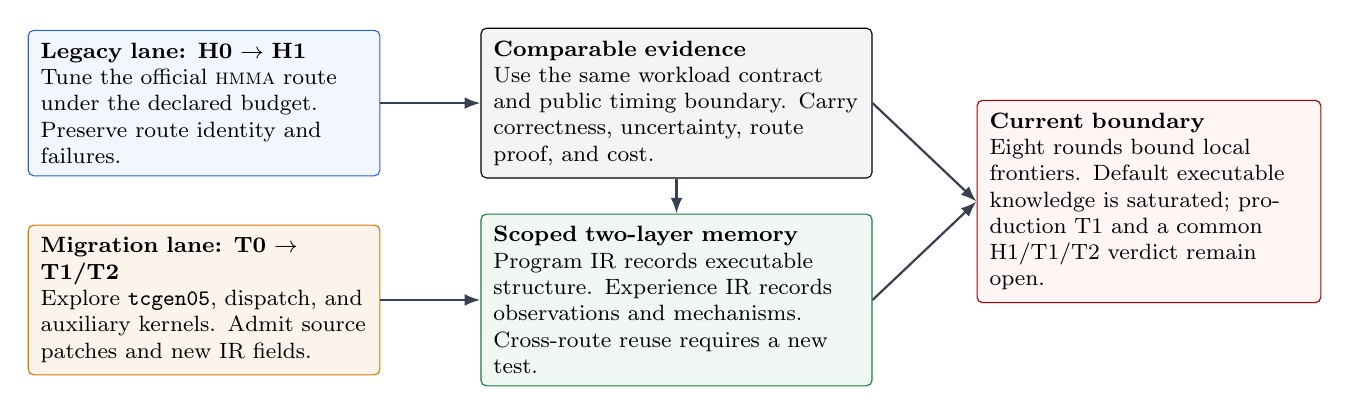
\begin{tikzpicture}[
  font=\footnotesize,
  box/.style={draw,rounded corners=2pt,inner sep=4.5pt,align=left},
  lane/.style={box,text width=4.15cm},
  centerbox/.style={box,text width=4.65cm},
  resultbox/.style={box,text width=4.05cm},
  arr/.style={-{Latex[length=2mm]},thick,darkgray}
]
\node[lane,draw=hmma,fill=hmma!6] (h) at (0,1.25) {\textbf{Legacy lane: H0 $\rightarrow$ H1}\\Tune the official \hmma{} route under the declared budget. Preserve route identity and failures.};
\node[lane,draw=tcgen,fill=tcgen!8] (t) at (0,-1.25) {\textbf{Migration lane: T0 $\rightarrow$ T1/T2}\\Explore \tcgen{}, dispatch, and auxiliary kernels. Admit source patches and new IR fields.};
\node[centerbox,fill=softgray] (g) at (6.0,1.25) {\textbf{Comparable evidence}\\Use the same workload contract and public timing boundary. Carry correctness, uncertainty, route proof, and cost.};
\node[centerbox,draw=irgreen,fill=irgreen!6] (ir) at (6.0,-1.25) {\textbf{Scoped two-layer memory}\\Program IR records executable structure. Experience IR records observations and mechanisms. Cross-route reuse requires a new test.};
\node[resultbox,draw=red!65!black,fill=red!4] (claim) at (12.0,0) {\textbf{Current boundary}\\Eight rounds bound local frontiers. Default executable knowledge is saturated; production T1 and a common H1/T1/T2 verdict remain open.};
\draw[arr] (h.east) -- (g.west);
\draw[arr] (t.east) -- (ir.west);
\draw[arr] (g.east) -- (claim.west);
\draw[arr] (ir.east) -- (claim.west);
\draw[arr] (g.south) -- (ir.north);
\end{tikzpicture}
\caption{The mainline challenge. Fair migration evidence requires two independently optimized lanes, a shared contract, and scoped transfer of experience. The current typed grammar accelerates execution but cannot define the full proposal space.}
\label{fig:challenge}
\end{figure}

\section{Why a closed search grammar is insufficient}

Early work typed one \tcgen{} coordinate: chunks assigned per prepare CTA. This rejected illegal values and enabled reproducible candidates, but risked confusing what the framework could express with what the kernel could improve.

The routes expose different transformations: \hmma{} may change warp layout, vector width, or decomposition; \tcgen{} may change tensor memory, roles, clusters, or compiler support. Evidence about \cpc{} is not evidence against these families.

MARPE therefore separates an \emph{open proposal plane} from an \emph{executable representation}. Each proposal receives one of four dispositions:
\begin{enumerate}
  \item \texttt{executable\_existing}: the current IR and evaluator can run it;
  \item \texttt{patch\_required}: a bounded source change can make it executable;
  \item \texttt{needs\_ir\_extension}: the idea is legitimate but the representation lacks a field or transform;
  \item \texttt{prototype\_first}: the mechanism should be tested by a small diagnostic before integration.
\end{enumerate}
Only malformed or out-of-contract proposals are rejected; representation gaps remain in the queue.

\section{Two-layer IR and proof-carrying evaluation}

\subsection{Program IR}

The program layer records the operator contract, route, architecture, source identity, schedule, guards, and compilation parameters. Its execution receipt includes the Python executable, package roots, \texttt{sys.path}, resolved modules and hashes, native extensions, selected CUDA sources and headers, target code generation, and relevant environment variables. It detects edits made in one checkout while another module or shared object executes.

Typed constraints enforce legal ranges, guards, and route compatibility before compilation; deterministic serialization gives every candidate a stable ID.

\subsection{Experience IR}

The experience layer stores each proposal, result, evidence and mechanism status, permitted use, and scope keys such as route, architecture, head count, workload, and phase. A timing win is an observation; its proposed cause becomes reusable only after phase attribution and a falsifiable transfer test.

Failures keep the same scope: an illegal carrier edit constrains that transformation, and a slower virtual-SM rule constrains those resource footprints. Transfer queries matching scope and mechanism, then validates anew.

\subsection{Deterministic gates}

Promotion follows fixed gates:
\begin{enumerate}
  \item establish route and build identity;
  \item test output and recurrent final-state correctness;
  \item time the complete public-call boundary with state reset;
  \item use paired ordering and record raw samples;
  \item estimate uncertainty and apply the registered decision rule;
  \item attribute the physical phase before writing a transferable mechanism;
  \item run a fresh held-out or prospective test before strengthening the claim.
\end{enumerate}
Agents supply hypotheses; deterministic gates decide the permitted claim. Search throughput cannot replace route verification, state correctness, or comparable measurement~\citep{kernelbench2025,asi2024,astra2025,kernelagent2026,kernelarc2026,kernelbenchverified2026}.

\section{Qualified \tcgen{} case study}

\subsection{Runtime profile and schedule}

The recurrent KDA call is described by a runtime profile
\[
P=(H,D,d_v,B,T,\tau,\mathcal{L},S,R),
\]
where $H$ is the head count, $D$ and $d_v$ are feature dimensions, $B$ is batch size, $T$ is total token count, $\tau$ is dtype, $\mathcal{L}$ is the sequence-length profile, $S$ is the physical SM count, and $R$ is the observed resident prepare-CTA count per SM. The studied Blackwell route launches a prepare kernel followed by a dependency-carrying chain kernel. The schedule parameter \cpc{} controls how many chunks each prepare CTA processes.

Let $W$ denote total chunks. For a fixed $H$, the prepare grid first fits in one resident wave when
\[
\cpc^*(W,H,S,R)=
\left\lceil
\frac{W}{\left\lfloor SR/H\right\rfloor}
\right\rceil .
\]
This equation is a physical hypothesis, not merely a fitted threshold. It predicts how the useful \cpc{} changes with work, head count, device capacity, and resource footprint.

\subsection{Measurement protocol}

Qualified measurements use the production public API on B300 compiled for \texttt{sm\_103a}. Every row checks output and recurrent final state, times the complete call with state reset, alternates candidate and baseline, and reports bootstrap intervals~\citep{efron1994bootstrap}. CUPTI attributes phases~\citep{cupti2026}; Nsight Compute checks resource assumptions~\citep{nsightcompute2026}.

\subsection{Evidence ladder}

Table~\ref{tab:qualified} summarizes the evidence. Moving \cpc{} from 4 to 9 improved two development calls by 1.0369$\times$ and 1.0807$\times$; CUPTI attributed 97.49--98.86\% of the reduction to prepare, supporting the wave mechanism.

The model predicted \cpc{} values 5, 9, and 17 for $W=256,512,1024$ at $H=12$, $S=148$, $R=5$; preregistered screens selected each winner and matched-work confirmations gained 1.0209--1.0859$\times$. It then prospectively chose 7 and 13 for $W=384,768$; four profiles gained 1.0133--1.1354$\times$, with weakest adjusted lower bound 1.0129. The capacity relation, rather than the constant 9, transferred.

\begin{table}[t]
\centering
\caption{Qualified B300 evidence for the \tcgen{} prepare policy. ``Prospective'' means the policy selected \cpc{} before candidate timing.}
\label{tab:qualified}
\small
\setlength{\tabcolsep}{4pt}
\begin{tabular}{@{}p{0.25\columnwidth}p{0.22\columnwidth}p{0.23\columnwidth}p{0.18\columnwidth}@{}}
\toprule
Stage & Profiles & Speedup & Evidence \\
\midrule
Development & fixed, mixed & 1.0369--1.0807 & paired CI \\
Mechanism & 4 profiles & 97.49--98.86\% & CUPTI attribution \\
Work scale & 4 profiles & 1.0209--1.0859 & predicted winners \\
Prospective & 4 profiles & 1.0133--1.1354 & adj. LB 1.0129 \\
\bottomrule
\end{tabular}
\end{table}

Short or highly split profiles do not benefit when prepare already fits or another phase dominates, so the policy remains guarded to its measured domain.

\section{Eight-round dual-lane campaign}

We ran eight falsification-first rounds with separate HMMA and tcgen05 queues. Rounds 1--7 gave each lane one challenger and two balanced GPU blocks; positive screens received four-block qualification. Round 8 allowed one structural hypothesis, one same-mechanism repair, three compiles, two correctness attempts, and two screen blocks per lane. The ledger matches present opportunities, not historical maturity; differing Round 8 scopes prohibit cross-lane latency comparison.

HMMA exposed a piecewise frontier. V64 beat V128 by 1.2172$\times$ and 1.1723$\times$ at H12 nseq 6, but fell below the 3\% gate at nseq 7--8. V32 beat V64 by 1.0764$\times$ at balanced nseq 3 and 1.0774$\times$ on a skewed holdout, yet regressed 3.82\% at nseq 4. The result is a CTA-wave crossover, not one best width. Lookahead depth 3 was bitwise correct but neutral to depth 2 (0.99998$\times$).

tcgen05 rejected a virtual-152-CTA rule on H64 and H96, then qualified H96 physical-148/s173 at 1.0330$\times$ over \cake{}. Grid147 gained 0.34\%, while TAIL4 and MINIMAX172 regressed. A constructively optimal maximum load of 169 still regressed by 6.17\%, proving that load minimax is not this carrier's latency objective.

Round 8 paired a full HMMA forward screen with a smaller tcgen05 V16 mechanism probe. Moving logical-B rematerialization outside the repeated lifecycle reduced registers 39 to 32 and static shared memory 9740 to 9228 bytes, preserved bitwise correctness, and ran 1.227$\times$ faster than scalar tcgen05 but 0.955$\times$ as fast as resident HMMA. It isolates layout cost without establishing a production P3/P4 or TMEM carrier.

\begin{table}[t]
\centering
\caption{Key dual-lane evidence. Q: four-block qualification; S: scoped screen or mechanism probe.}
\label{tab:probe}
\small
\setlength{\tabcolsep}{4pt}
\begin{tabular}{@{}p{0.16\columnwidth}p{0.31\columnwidth}p{0.34\columnwidth}p{0.10\columnwidth}@{}}
\toprule
Lane & Intervention & Result & Status \\
\midrule
HMMA & V32/V64, balanced nseq 3 & 1.0764$\times$ & Q \\
HMMA & V32/V64, balanced nseq 4 & 0.9618$\times$ & S \\
HMMA & lookahead L3/L2 & 0.99998$\times$ & S \\
tcgen05 & H96 s173/\cake{} & 1.0330$\times$ & Q \\
tcgen05 & load-optimal 169/default & 0.9383$\times$ & S \\
tcgen05 & preferred/scalar probe & 1.227$\times$ & S \\
tcgen05 & preferred/HMMA probe & 0.955$\times$ & S \\
\bottomrule
\end{tabular}
\end{table}

An H96 request silently fell back to \cake{}, a fresh-seed H12 \cake{} arm failed correctness, and an HMMA call used an incompatible binding. The rows were excluded or repaired within budget, motivating first-class module paths, hashes, symbols, launches, and failures.

\section{Agent architecture and research memory}

\paragraph{Open-source provenance.}
MARPE is an integration and domain adaptation, rather than a multi-agent system implemented from scratch. Its search plane reuses PIKE-B's independent initial proposals, parallel branches, repair agents, candidate allocation, and top-branch selection~\citep{pike2025}. Its execution and evidence plane reuses Atrex Kernel Agent's isolated GPU execution, NVIDIA profiling, Git-worktree episodes, resumable journals, and incumbent/candidate ABBA verification~\citep{atrex2026}. The artifact vendors audited snapshots at PIKE revision \texttt{fd5721e9} under MIT and Atrex revision \texttt{d643fb5b} under Apache-2.0, with upstream notices retained.

\paragraph{Contribution and experimental boundary.}
The work introduced here is the FlashKDA-specific control plane: separate HMMA and tcgen05 Program IRs, scope-keyed Experience IR, a matched-opportunity budget protocol, and proof-carrying candidate promotion. These additions keep route-specific legal transformations separate while making correctness, execution identity, uncertainty, and permitted claim scope authoritative. The present experiment is a narrow-width dual-branch loop, with one new challenger per lane in Rounds 1--7 and one structural hypothesis per lane in Round 8. We did not run a matched single-agent ablation, so the results do not establish that multi-agent search outperforms a single agent; they establish the behavior of this attributed integration on the migration case study.

MARPE uses roles to diversify hypotheses, not to vote on truth. A scout inspects source and profiles bottlenecks. A proposer emits typed or source-identified edits. A falsifier searches for counterexamples and route mistakes. An evaluator runs deterministic gates. A synthesizer writes scoped experience entries and updates the proposal queue. Roles may operate concurrently, while promotion and memory writes remain serialized by candidate identity.

The campaign allocates matched opportunity caps to the two lanes: proposal, repair, compile, correctness, screen, and qualification slots are frozen before execution. Failed builds and wrong-route runs consume their slots. Within a lane, schedule parameters, source transformations, dispatch policies, and representation extensions compete in one ledger. Search cost remains separate from historical code maturity and code size; equal present-day opportunities cannot erase different starting maturity. When evidence scopes differ, as in a public extension and a mechanism probe, the ledger compares exploration opportunity rather than latency.

Experience reuse follows three rules. First, transfer invariants such as route verification, state reset, and execution receipts broadly. Second, transfer mechanism hypotheses only when their variables exist on the destination route. For example, resident-wave reasoning may transfer, while the fitted H12 \cpc{} value does not. Third, treat contradictions as scope refinement. When H12 and H96 disagree, memory should split by resource footprint or route phase instead of overwriting one result.

This structure avoids two common agent failures. A memory system that stores only winners repeats unsafe attempts because it loses the boundary of legality. A memory system that globalizes every failure suppresses new ideas because one route's constraint becomes another route's false prohibition. Scoped program and experience IR provide a middle ground: agents inherit concrete evidence while the proposal plane stays open.

\section{What the current evidence establishes}

The evidence supports five claims. First, runtime profile belongs in the optimization representation: one compiled operator needs different physical schedules and vector widths at different work scales. Second, proof-carrying evaluation catches route fallback, stale modules, incompatible bindings, and correctness failures that timing alone misses. Third, mechanism-backed memory transfers better than constants: the resident-grid equation predicted new work scales, whereas virtualizing the SM count failed. Fourth, legacy exploration is necessary because H0 was materially improvable and its dispatch frontier was piecewise. Fifth, a theoretical optimum in one IR coordinate need not optimize latency: the exact load-minimax schedule was substantially slower.

Within the frozen B300, existing-carrier envelope, an independent proposal audit found no new high-value executable family. HMMA vector-width and lookahead hypotheses have scoped boundaries; tcgen05 grid, task-grouping, load-minimax, and one-time preferred-layout hypotheses have direct evidence. We call this \emph{default-knowledge high-value proposal saturation}, not a hardware or algorithmic optimum. Cheap unmotivated variants remain possible, but repeating them would not add a new mechanism.

The headline migration verdict remains open because the strongest tcgen05 structural idea now requires information outside the envelope: a lane-verified P3/P4 preferred-layout producer, an explicit BF16 rounding boundary, or cross-phase TMEM residency. The tcgen05 probe cannot stand in for production T1, and its latency cannot be compared with the HMMA public-forward screen. The next decisive work is evidence closure: build that carrier, freeze common profiles and the public-call boundary, and qualify H1, T1, and T2 with paired uncertainty. A global optimum would additionally require a tight latency lower bound.

\section{Related work}

TensorIR, Ansor, and MetaSchedule use structured program representations to define legal search spaces~\citep{tensorir2023,ansor2020,metaschedule2022}. Triton and CUTLASS expose reusable GPU scheduling and tensor-core abstractions~\citep{triton2019,cutlass2026}. Stream-K shows why work decomposition and occupancy interact with shape and device scale~\citep{streamk2023}. MARPE focuses on an operational gap: a production migration may require proposals outside the current grammar, and every reported win must remain tied to the route, environment, and public-call contract that produced it.

Recent kernel agents broaden candidate generation through language models, evolutionary search, and iterative feedback~\citep{asi2024,astra2025,kernelagent2026,kernelarc2026}. Our contribution is complementary. We use agents to explore an open proposal plane, while deterministic evidence gates and scoped memory control what becomes reusable knowledge. This separation is especially useful when two architectural routes have different legal transformations and maturity.

\section{Conclusion}

The FlashKDA migration question cannot be resolved by optimizing \tcgen{} against an untouched \hmma{} baseline. It requires two independently optimized lanes, a shared contract, and evidence that records exactly what executed. MARPE combines an open proposal plane with typed program IR, scoped experience IR, and proof-carrying promotion. Eight B300 rounds qualified a profile-dependent HMMA dispatch improvement, rejected a mathematically optimal but slower tcgen05 load schedule, and isolated a preferred-layout cost without overstating a microprobe as T1. Existing-carrier high-value proposal generation is now saturated under the frozen envelope. The remaining work changes the representation itself: construct the production tcgen05 carrier, then earn the common-profile H1/T1/T2 verdict.

{\small
\bibliographystyle{unsrtnat}
\bibliography{references}
}

\end{document}
